A microgrid similar to the one shown in Fig \ref{fig:system_arch} is constructed using the load and solar data collected form a Florida feeder available in the SUNGRIN project \cite{SUNGRIN} for testing the algorithm described in Section \ref{A*}. Table \ref{tab:solar_pv} shows the physical parameters of the PV plant and its inverter. The physical parameters of the energy storage used are shown in table \ref{tab:es}. The levelized cost of energy (LCOE)  of the energy storage system $R_{ESS}$ is calculated using equation \ref{eq:R_ESS}.

\begin{equation}
\label{eq:R_ESS}
R_{ESS} = \dfrac{ES_{tot}}{Cyc\cdot ES_{Cap}\cdot DoD\cdot \eta_{r}},
\end{equation}

%%%%%%%%PV%%%%%%%%%%%%%%%%%%%%%%%%%%%%%%%%%%%
\begin{table}[htb]
\normalsize
\renewcommand{\arraystretch}{1}
\caption{PV System Specifications}
\label{tab:solar_pv}
\centering
    \begin{tabular}{ | l | p{3cm} | }
    \hline
    \textbf{PV System Parameters} & \textbf{Value} \\ \hline
    PV Panels Rating (\(P_{PV}\)) & 875 kW  \\ \hline
    Inverter Rating (\(S_{PV}\)) & 900 kVA \\ \hline
    Power Factor Range (\(pf_{PV}\)) & 0.8-1.0  \\ \hline
    Max. Reactive Power (\(\overline{Q_{PV}}\)) & 540 kVAR \\ \hline
    Min. Reactive Power (\(\underline{Q_{PV}}\)) & -540 kVAR \\ \hline
    LCOE (\(r_{PV}\)) & 2.51 c/kWh \\ \hline
    \end{tabular}
    \begin{tabular}{l}
    \end{tabular}
\end{table}
%%%%%%%%PV%%%%%%%%%%%%%%%%%%%%%%%%%%%%%%%%%%%


%%%%%%%%ES%%%%%%%%%%%%%%%%%%%%%%%%%%%%%%%%%%%
\begin{table}[htb]
\normalsize
\renewcommand{\arraystretch}{1}
\caption{Energy Storage (ES) System Specifications}
\label{tab:es}
\centering
    \begin{tabular}{ | l | p{3cm} | p{3cm} | }
    \hline
    \textbf{ES System Parameters} & \textbf{Value} \\ \hline
    ES Rating (\(P_{ES}\)) & 750 kW  \\ \hline
    Inverter Rating (\(S_{ES}\)) & 750 kVA \\ \hline
    Max. State of Charge  (\(\overline{SOC_{ES}}\)) & 2190 kWh \\ \hline
    Min. State of Charge  (\(\underline{SOC_{ES}}\)) & 219 kWh \\ \hline
    Power Factor Range (\(pf_{ES}\)) & 0.8-1.0  \\ \hline
    Max. Reactive Power (\(\overline{Q_{ES}}\)) & 450 kVAR \\ \hline
    Min. Reactive Power (\(\underline{Q_{ES}}\)) & -450 kVAR \\ \hline
    LCOE (\(r_{ES}\)) & 12.3 c/kWh \\ \hline
    \end{tabular}
\end{table}
%%%%%%%%ES%%%%%%%%%%%%%%%%%%%%%%%%%%%%%%%%%%%

The load and solar profile for the testing of the algorithm were obtained from the SUNGRIN project. Fig \ref{fig:LOAD_PROFILE_8} shows the load profile of the system for eight days with average, minimum and maximum loads.

\begin{figure}[!ht]
    \centering
    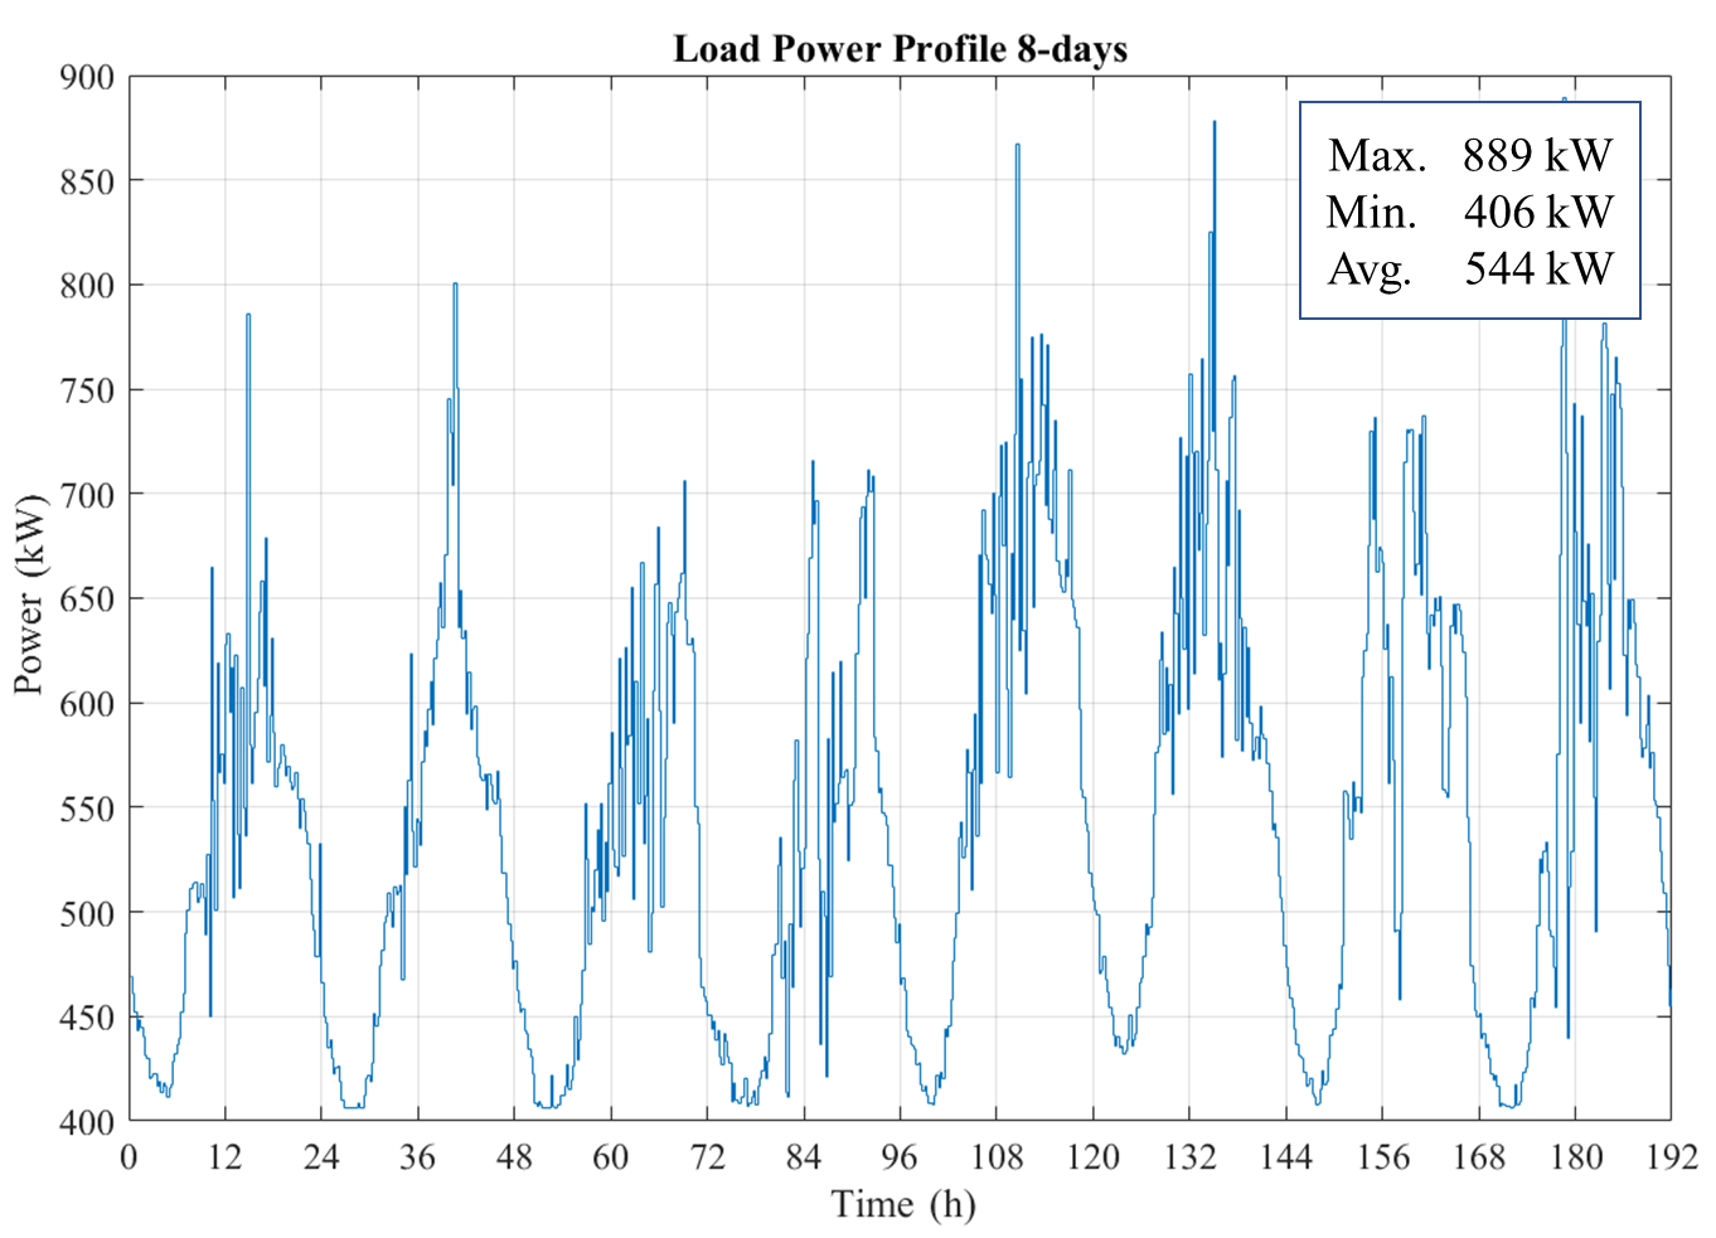
\includegraphics[width = \linewidth]{figs/loadprofile.png}
    \caption{Eight day load profile}
    \label{fig:LOAD_PROFILE_8}
\end{figure}

To generate the RTP profile Locational Based Marginal Pricing (LBMP) data is collected from the New York Independent System Operator (NYISO) \cite{NYISO2017}. The collected LBMPO is combined with the time of use price available at Tallahassee to generate a RTP for the test case. Fig \ref{fig:RTP_PROFILE_8} shows the real-time price profile used for the test system. The system is also tested against time of use pricing scheme available from PG\&E \cite{pgne}. Fig \ref{fig:PGNE_PRICE} shows the price profile acquired from PG\&E.

\begin{figure}[!ht]
    \centering
    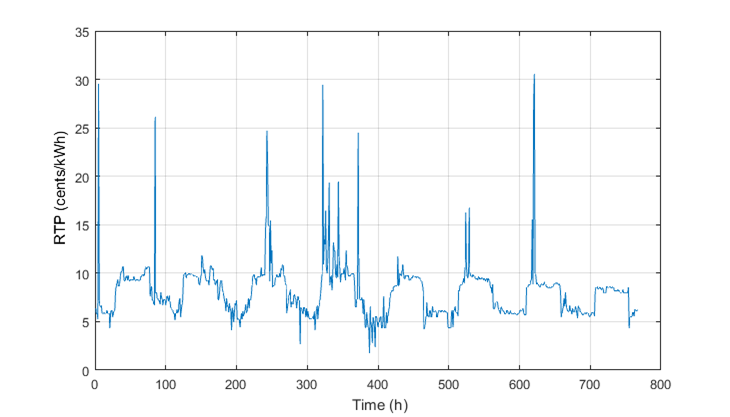
\includegraphics[width = \linewidth]{figs/rtp_8days.png}
    \caption{Eight day RTP profile NYISO}
    \label{fig:RTP_PROFILE_8}
\end{figure}

\begin{figure}[!ht]
    \centering
    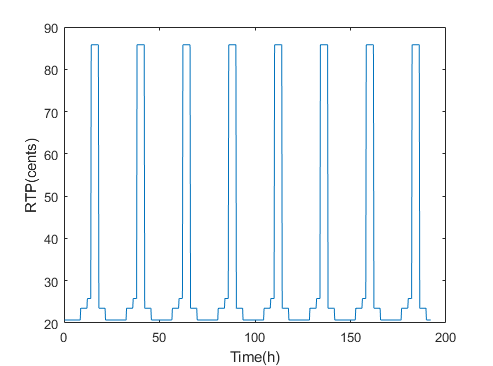
\includegraphics[width = \linewidth]{figs/PGNE_PRICE.png}
    \caption{Eight day RTP profile PG\&E}
    \label{fig:PGNE_PRICE}
\end{figure}

The PV profile used in the system is collected from the SUNGRIN project and scaled to fit the ratings of the PV described in table \ref{tab:solar_pv}. Fig \ref{fig:PV_PROFILE_8} shows the eight-day PV profile used.

\begin{figure}[!ht]
    \centering
    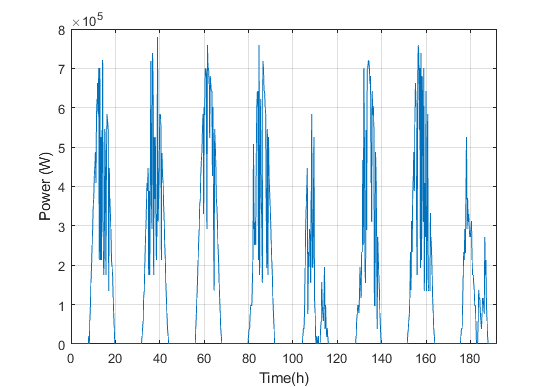
\includegraphics[width = \linewidth]{figs/PV_PROFILE.png}
    \caption{Eight day PV profile}
    \label{fig:PV_PROFILE_8}
\end{figure}